\section{Amélioration}

	Dans le but de simplifier l'expérience de l'utilisateur, nous avons souhaité ajouter certaines fonctionnalités à notre logiciel. Si celles-ci n'apportent pas d'amélioration en terme d'analyse des arbres, elles permettent de faciliter grandement leur modification. Nous distinguerons deux types de modifications : celles qui simplifient l'édition de l'arbre par l’intermédiaire d'AdTool, qui se traduiront par une modification de ce logiciel, et celles intégrées à \textbf{Glasir} qui simplifieront la navigation entre les différents arbres (qu'ils soient réalisés par l'utilisateur lui-même ou importés comme modèles). 

	\subsection{Liste d'arbres}.

	Dans sa version actuelle, ADTool ne permet d'ouvrir qu'un seul arbre à la fois : cette limitation est particulièrement handicapante. Par exemple, l'utilisateur ne peut pas ouvrir deux versions différentes d'un même arbre pour les comparer. Notre logiciel rendra donc possible l'ouverture simultanée de plusieurs onglets, chacun possédant un arbre différent. 

	Cette fonctionnalité induit la possibilité pour l'utilisateur de manipuler un grand nombre d'arbres en simultané dans le cadre d'un même projet. Le module \emph{Liste d'arbres} fournira à l'utilisateur une présentation de la liste des arbres du projet sous forme d'arborescence. Il s'agira d'un dock disponible sur le côté du logiciel. 

	L'utilisateur aura aussi la possibilité de créer des catégories et des sous-catégories d'arbres pour hiérarchiser son projet. La suppression, la création et le renommage d'un arbre seront réalisables directement depuis ce module.
	
	\subsection{Bibliothèque de modèles}

	Il n'est pas toujours aisé pour l'utilisateur de créer un arbre en partant de rien. C'est pourquoi \emph{Glasir} fournira à l'utilisateur une bibliothèque de modèles, chacun pouvant servir de base pour de nouveaux arbres. Cette bibliothèque contiendra un ensemble d'arbres génériques, que l'utilisateur pourra personnaliser et compléter pour créer un nouvel arbre. Il pourra aussi l'utiliser tel quel s'il lui convient. La création d'un nouveau projet entraînera une copie de la bibliothèque de modèles de base, qui pourra ensuite être modifiée par l'utilisateur. Une bibliothèque de modèles est donc propre à chaque projet. Par exemple, si l'expert crée un arbre qu'il juge utile de réexploiter plusieurs fois dans le projet, il lui sera possible de l'intégrer à la bibliothèque de modèles.

	\subsection{Éditeur d'arbres}

	L'édition des arbres dans \emph{Glasir} se fera exclusivement par l'intermédiaire d'ADtool. L'ouverture d'un arbre par l'utilisateur provoque le lancement d'une instance d'ADTool contenant cet arbre. ADTool n'offrant pas la possibilité d'ouvrir plusieurs arbres à la fois, chaque instance (une par arbre) est imbriquée dans l'IHM du logiciel sous la forme d'onglet. Pour rendre possible l'interaction entre \emph{Glasir} et ADtool, nous apporterons quelques modifications à ce dernier, qui seront explicitées par la suite.

\subsection{Couper/copier/coller}
	
	Actuellement, ADTool ne permet pas l'utilisation des fonctions couper/copier/coller qui pourraient pourtant s'avérer pratiques lors de la création d'un arbre. Par exemple, dans le cas de l'oubli d'un nœud père, l'instauration de ces fonctionnalités permettra de déplacer facilement les fils concernés de l'ancien nœud père vers le nouveau.\\
	En conséquence, la sélection d'un nœud entraînera la sélection de ses fils, afin de pouvoir effectuer des transferts rapidement. Ceci sera automatique, car nous avons considéré que la sélection partielle des nœuds fils ne présentait pas vraiment d'utilité. Le système de raccourcis clavier classique ne sera probablement pas repris, au profit d'une gestion à la souris et d'un affichage spécial des nœuds copiés (coloration particulière, par exemple).\\

	Cependant, cette fonctionnalité entraîne des questions de cohérence. En effet, des nœuds de même label ne pourront pas être présents, il faudra donc gérer ces cas de figure. L'édition XML abordée ci-dessous sera le moyen le plus simple de résoudre ces éventuels conflits.

	\subsection{Amélioration du codage des arbres}

	Tel qu'il existe aujourd'hui, ADTool affiche dans son interface une section nommée \emph{ADTerm Edit}. Celle-ci affiche une représentation de l'arbre sous un format texte, en utilisant un langage propre au logiciel. Lors de la modification de l'arbre dans l'éditeur graphique, AdTool met à jour le texte correspondant en temps réel et de manière automatique. L'inverse est également vrai : il est possible de changer les labels des nœuds, ou les opérateurs, directement depuis \emph{ADTerm Edit} puis afin d'afficher le résultat graphiquement (après validation).\\ 

	Mais le langage qui permet de décrire les arbres sous format texte n'est pas très lisible : par exemple, il ne contient pas le nom des nœuds autres que les feuilles. Sur la figure \ref{fig:int_adTool}, on peut constater que le code indique le nom des deux feuilles \textit{Acheter le matériel nécessaire} et \textit{Essayer les clés de chiffrage}, que la conjonction est bien précisée par l'opérateur \textit{ap}, mais qu'aucune référence n'est faite au label du nœud parent (\textit{Casser le chiffrage}). Pour remédier à ce problème, nous créerons une nouvelle grammaire corrigeant ce défaut afin de rendre l'utilisation de cette fenêtre plus intuitive.\\
	
	Cependant, cette représentation des arbres doit rester facultative, l'utilisateur pouvant juger l'interface graphique suffisante pour effectuer des modifications. C'est pour cette raison que nous voulons aussi ajouter la possibilité de masquer la section \emph{ADTerm Edit}, ce qui permettrait de gagner de la place pour afficher les arbres graphiquement.

	% ATTENTION  !! CHANGER CRIPTAGE EN CHIFFFRAGE !!!
	\begin{figure}
		\centering
		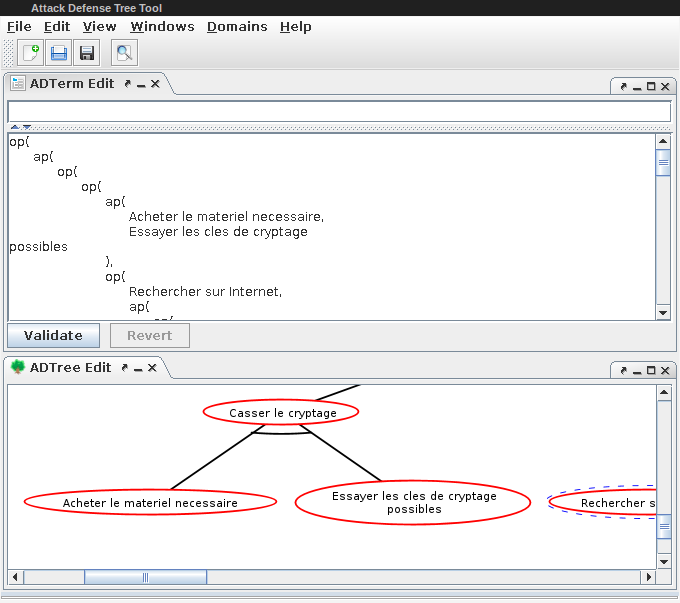
\includegraphics[width=0.5\textwidth]{figure/interface_adtool.png}
		\caption{L'interface d'AdTool.}
		\label{fig:int_adTool}
	\end{figure}
	
	\subsection{CTRL-Z}
	
	Pour le moment, effectuer une action sous ADTool est irréversible. Cela n'est pas grave pour certaines actions rapides à effectuer, telles que le renommage d'un nœud. Mais supprimer un nœud (implique la disparition de tous ses nœuds fils s'il y en a) par erreur peut entraîner un travail énorme, et donc une perte de temps. La possibilité de revenir à l'état précédent de l'arbre éviterait d'avoir à refaire ce travail de construction fastidieux. Nous souhaitons créer au moins une sauvegarde de l'état précédent, afin de pouvoir annuler la dernière modification. Si possible, nous envisageons l'implémentation d'une pile circulaire contenant les N derniers états (chaque modification entraînant la création d'un nouvel état) avec un curseur pointant sur l'état courant. Cela permettrait de revenir en arrière sans contraintes.

	\subsection{Vue globale des paramètres}
	
	Dans l'état actuel d'ADTool, lorsqu'un arbre est valué, un seul paramètre est affiché (le même pour tous les nœuds) même si plusieurs paramètres sont utilisés en réalité. En effet, chaque valuation a un onglet propre, et un dans lequel elle est la seule effectivement affichée sur l'arbre. Nous souhaitons créer un onglet plus général, dans lequel tous les paramètres appliqués peuvent être visibles sur l'arbre. C'est ensuite à l'expert de décider des paramètres qu'il juge utile d'afficher. Cela faciliterait aussi la création des paramètres de synthèse évoqués précédemment.\\
	
	Pour une meilleure lisibilité, chaque paramètre aura une couleur différente, et l'arbre sera accompagné d'une légende résumant ce jeu de coloration et ses correspondances. Nous devrons également gérer la taille des nœuds, pour que les paramètres ne dépassent pas de la bulle. Un tel système étant déjà présent dans ADTool pour gérer les labels, il suffira de l'étendre à l'affichage des paramètres.
